\chapter{Inferenz und Resolution}
\label{chap:inferenz_resolution}

\section{Inferenz}
\label{sec:inferenz}
Grundsätzlich geht es bei Inferenz um den Prozess von Schlussfolgerungen mithilfe von Resolution (siehe~\ref{sec:resolution}). Die logische Inferenz ist ein Prozess der Inferenz und Resolution, welcher die Folgebeziehungen zwischen Sätzen zum Ausdruck bringt.~\cite[S. 163]{russel}.

\subsection{Inferenz in Computern}
\label{subsec:inferenz-in-computer}

Das grundsätzliche Problem bei Computern im Bezug auf Inferenz ist, dass ein Computer keine Interpretation vornehmen kann und nichts über die (Um-) Welt weiss, bzw.\ nur, was in seiner Wissensdatenbank gespeichert ist (vgl.~\citet[S. 164]{russel}).


Angenommen, man möchte einen Computer fragen

\lstset{caption={Beispielanfrage an eine Wissensdatenbank eines Computers},captionpos=b}
\begin{lstlisting}
    ``Ist eine Abenteuerreise eine Reise?''
\end{lstlisting}

so weiss der Computer weder was ein Abenteuerreise ist, noch kennt er das Konzept des Reisens an sich. Das Einzige, was er tun kann, ist, in der Wissensdatenbank nach 

\lstset{caption={Aussage in einer Wissensdatenbank eines Computers},captionpos=b}
\begin{lstlisting}
    ``Eine Abenteuerreise ist eine Reise.''
\end{lstlisting}

zu suchen. Findet der Computer diese Aussage in der Wissensdatenbank, so spielt es keine Rolle, dass er das Konzept der Abenteuerreise oder des Reisens nicht kennt. Die Schlussfolgerung, dass eine Abenteuerreise eine Reise ist, trifft unter allen Gegebenheiten und Interpretationen zu, welche für die Wissensdatenbank zutreffen (vgl.~\cite[S.164]{russel}).

Zusammengefasst kann gesagt werden, dass die formale Inferenz in der Lage ist, gültige Schlussfolgerungen zu ziehen, auch wenn der Computer die Interpretationen des Anwenders nicht kennt. Der Computer zieht immer logisch gültige Schlüsse, unabhängig von der (menschlichen) Interpretation. Da der Mensch in der Regel die Interpretation kennt, erscheinen die Schlüsse dem Menschen logisch (vgl.~\cite[S. 165]{russel}).

\section{Resolution}
\label{sec:resolution}

Resolution, aus dem Lateinischen ``resolutio'', zu Detsch ``Auflösung'', ist eine Verallgemeinerung des Modus Ponens~\cite[S. 279]{russel}. Die Methode der Resolution wurde 1965 von J. A. Robinson entwickelt, dabei handelt es sich um einen vollständigen Algorithmus der Theorembeweisung für Prädikatenlogik erster Stufe.~\cite[S. 18]{russel} In der einfachsten Form handelt es sich bei der Resolution um eine Inferenz-Regel der Aussagenlogik.~\cite[S. 277]{russel}

Eine Verallgemeinerung der einfachen Form der Inferenz-Regel zur Resolution kann als Regel zur kompletten Inferenz der Prädikatenlogik erster Stufe genutzt werden.~\cite[S. 278]{russel}

\section{Praktische Umsetzung}
\label{sec:inferenz_praktisch}

Inferenz im semantischen Netz kann grundsätzlich als das Entdecken von neuen Beziehungen zwischen Entiäten beschreiben werden. Dies heisst, dass automatische Prozeduren, in Form von so genannten \textit{Reasonern}, neue Beziehungen generieren. Wie die neuen Beziehungen umgesetzt werden --- durch Hinzufügen zu den Daten oder durch eine einfach Rückgabe dieser --- ist eine Frage der Implementation (vgl.~\cite[Abschnitt 1]{w3inference}). Eine detaillierte Beschreibung solch einer praktischen Umsetzung, in Form des \textit{Pellet} Reasoners der Firma Clark \& Parsia, findet sich unter.%TODO: ~\ref{THESIS-sec:komponenten}.

\subsection{Beispiel}
\label{subsec:inferenz_beispiel}

Gegeben seien folgende Datensätze, welche Regeln definieren

\begin{lstlisting}[caption={Aussagentripel bestehend aus Objekt, Prädikat und Subjekt},captionpos=b,label=lst:reasoning_seilpark]
    ``Schweiz hatRegion Solothurn.''
    ``Solothurn hatOrt Balmberg.''
    ``Seilpark istUnterklasseVon Ausflug.''
    ``Seilpark hatStandort Balmberg.''
\end{lstlisting}

definiert.

Unterstützt nun ein Programm Inferenz, z.B. durch einen Reasoner, so kann dieser schlussfolgern, dass der Ausflug \textit{Seilpark} in der Region Solothurn ist (vgl.~\cite[Abschnitt `Examples']{w3inference}).

\newpage

\noindent\rule[1ex]{\textwidth}{1pt}
\begin{wrapfigure}[14]{l}{0.1\textwidth}
    \vspace{-12pt}
    
\includegraphics[width=0.1\textwidth]{bilder/elephant.png}
\end{wrapfigure}
Das unter~\ref{lst:reasoning_seilpark} genannte Beispiel beantwortet genau die unter~\ref{sec:wissensrepFormen_Wissensnetze} gestellte Frage, wie man zum Schluss gelangt, dass das Individuum \textit{Seilpark Balmberg} in der \textit{Region} \textit{Solothurn} ist.

Wie wendet man dies jedoch an? Wie gelangt man effektiv zu dieser Information? Kann dies effektiv durch reine Folgerung erreicht werden?

Die Antwort hierzu lautet ja und nein. Modelliert man die Situation beispielsweise in Protégé und nutzt den Pellet-Reasoner zum Ziehen von Schlüssen, so würde man annehmen, dass dies der Fall ist. Rein von den Möglichkeiten her sollte der Reasoner genau dies bieten. Dies ist jedoch nicht ganz der Fall, wie in der nachfolgenden Grafik ersichtlich ist.

\begin{figure}[H]
\centering \rotatebox{0}{\scalebox{0.5}[0.5]{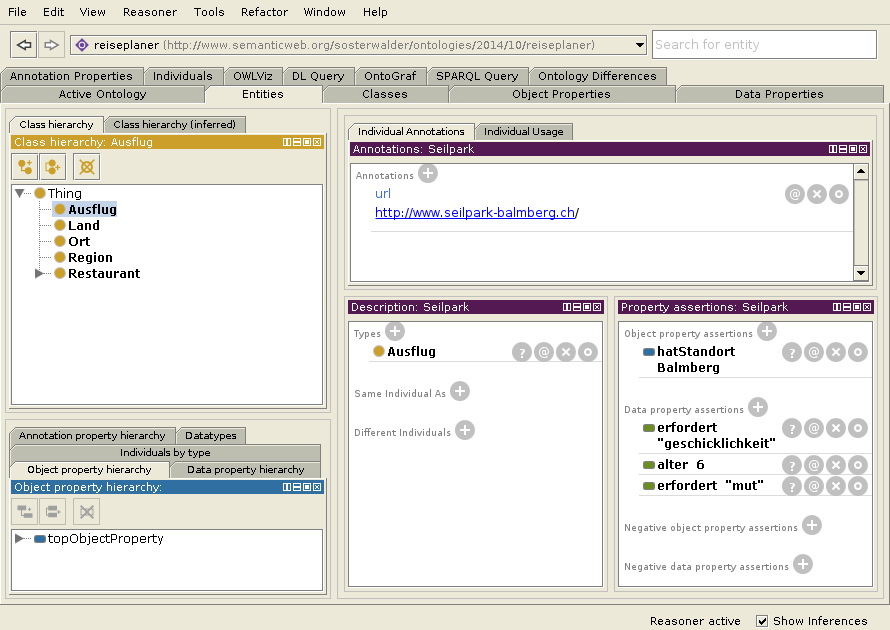
\includegraphics{bilder/inferenz_protege.png}}}
\caption{Darstellung des Individuums \textit{Seilpark Balmberg} in Protégé.\label{fig:inferenz_protege}\protect\footnotemark}
\end{figure}
\footnotetext{Eigene Darstellung mittels Stanford Protégé Version 5.0.0 beta 15}

Eine solche Folgerung ist durchaus möglich, man muss den Relationen die entsprechenden Eigenschaften, wie Symmetrie oder Transivität, geben. Wir haben dies in unserem Fall jedoch bewusst nicht getan, da sonst Folgerungen auftreten, welche irreführend sind, so wäre dann z.B. ein Ort auch ein Land und umgekehrt.

Wir haben die eigentliche Folgerung mittels einer Regel in der Ontologie vorgenommen. Dies führen wir zu einem späteren Zeitpunkt noch genauer aus.

\noindent\rule[1ex]{\textwidth}{1pt}
